Use Venn diagrams to verify the following identities:
\begin{enumerate}[label=(\alph*)]
    \item $(A \cup B) \: \backslash \: C = (A \: \backslash \: C) \cup (B \: \backslash \: C)$.
    \item $A \cup (B \: \backslash \: C) = (A \cup B) \: \backslash \: (C \: \backslash \: A)$.
\end{enumerate}

\textbf{Solution:}
\begin{enumerate}[label=(\alph*)]
    \item Elements in the union of $A$ and $B$ and none in $C$.\\
        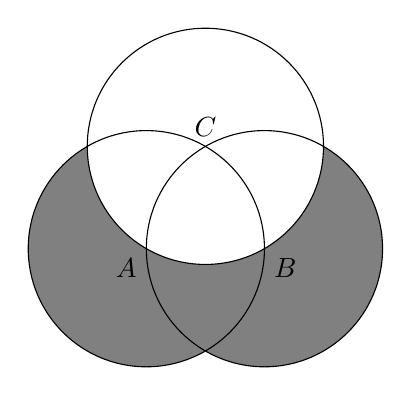
\begin{tikzpicture}
          % Define circles for A, B, and C
          \def\circleA{(0,0) circle (1.5cm)}
          \def\circleB{(1.5,0) circle (1.5cm)}
          \def\circleC{(0.75,1.3) circle (1.5cm)} % Positioned to overlap both A and B
        
          % Draw and fill A union B excluding C
          \begin{scope}
            \clip \circleA \circleB; % Clip to union of A and B
            \fill[gray] \circleA \circleB;
            \clip \circleC; % Clip further to C
            \fill[white] \circleA \circleB; % Fill intersection with C in white
          \end{scope}
          
          % Outline the circles and label them
          \draw \circleA node [text=black, below left] {$A$};
          \draw \circleB node [text=black, below right] {$B$};
          \draw \circleC node [text=black, above] {$C$};
        \end{tikzpicture}

    \item Elements in the union of $A$ and unique to $B$.\\
        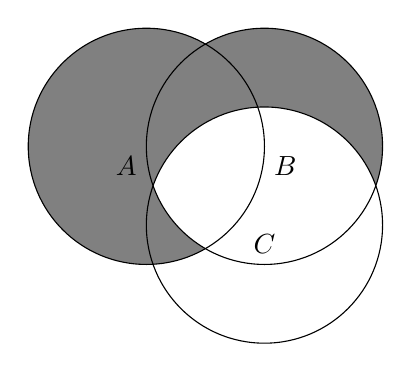
\begin{tikzpicture}
          % Define circles for A, B, and C
          \def\circleA{(0,0) circle (1.5cm)}
          \def\circleB{(1.5,0) circle (1.5cm)}
          \def\circleC{(1.5,-1) circle (1.5cm)} % Positioned to overlap only with B
        
          % Fill A completely
          \fill[gray] \circleA;
        
          % Fill B excluding C
          \begin{scope}
            \clip \circleB;
            \fill[gray] \circleB;
            \clip \circleC;
            \fill[white] \circleB;
          \end{scope}
        
          % Outline the circles and label them
          \draw \circleA node [text=black, below left] {$A$};
          \draw \circleB node [text=black, below right] {$B$};
          \draw \circleC node [text=black, below] {$C$};
        \end{tikzpicture}
\end{enumerate}
\pagebreak